\documentclass{beamer}
\usepackage[utf8]{inputenc}
\usetheme{Madrid}
\usecolortheme{default}
\usepackage{amsmath,amssymb,amsfonts,amsthm}
\usepackage{txfonts}
\usepackage{tkz-euclide}
\usepackage{listings}
\usepackage{adjustbox}
\usepackage{array}
\usepackage{tabularx}
\usepackage{gvv}
\usepackage{lmodern}
\usepackage{circuitikz}
\usepackage{tikz}
\usepackage{graphicx}

\setbeamertemplate{page number in head/foot}[totalframenumber]

\usepackage{tcolorbox}
\tcbuselibrary{minted,breakable,xparse,skins}



\definecolor{bg}{gray}{0.95}
\DeclareTCBListing{mintedbox}{O{}m!O{}}{%
  breakable=true,
  listing engine=minted,
  listing only,
  minted language=#2,
  minted style=default,
  minted options={%
    linenos,
    gobble=0,
    breaklines=true,
    breakafter=,,
    fontsize=\small,
    numbersep=8pt,
    #1},
  boxsep=0pt,
  left skip=0pt,
  right skip=0pt,
  left=25pt,
  right=0pt,
  top=3pt,
  bottom=3pt,
  arc=5pt,
  leftrule=0pt,
  rightrule=0pt,
  bottomrule=2pt,
  toprule=2pt,
  colback=bg,
  colframe=orange!70,
  enhanced,
  overlay={%
    \begin{tcbclipinterior}
    \fill[orange!20!white] (frame.south west) rectangle ([xshift=20pt]frame.north west);
    \end{tcbclipinterior}},
  #3,
}
\lstset{
    language=C,
    basicstyle=\ttfamily\small,
    keywordstyle=\color{blue},
    stringstyle=\color{orange},
    commentstyle=\color{green!60!black},
    numbers=left,
    numberstyle=\tiny\color{gray},
    breaklines=true,
    showstringspaces=false,
}
%------------------------------------------------------------
%This block of code defines the information to appear in the
%Title page
\title %optional
{9.3.8}

%\subtitle{A short story}

\author % (optional)
{BALU-ai25btech11017}



\begin{document}


\frame{\titlepage}
\begin{frame}{Question}
Find the area of the region $\{(x, y) : x^2 \leq y \leq x\}$.
\\ 
\end{frame}
\begin{frame}{Theoretical Solution}
Let us solve the given equation theoretically and then verify the solution computationally \\
According to the question, \\
equation line
\begin{align}
\vec{x}=\lambda\myvec{1\\1}
\end{align}
equation of parabola is
\begin{align}
   \vec{x}^T\vec{v}\vec{x}+2\vec{u}^T\vec{x}+f=0
\end{align}
where
\begin{align}
   \vec{v}=\myvec{1&&0\\0&&0}\\
   \vec{u}=\myvec{0\\\frac{-1}{2}}\\
   f=0
\end{align}
\end{frame}
\begin{frame}{Theoretical Solution}
substute 0.1 in 0.2\\
$\lambda=0,1$ so intersection points are
\begin{align}
   \vec{a_1}=\myvec{0\\0}\\
   \vec{a_2}=\myvec{1\\1}\
\end{align}
hence the requried area is
\begin{align}
    \int_{0}^{1} (x-x^2) \, dx=\frac{1}{6}
\end{align}
\end{frame}
\begin{frame}[fragile]
    \frametitle{C Code}

    \begin{lstlisting}
 #include <stdio.h>

int main() {
    // Conic: y = x^2
    double V[2][2] = {{1, 0}, {0, 0}};
    double u[2] = {0, -0.5};
    double f = 0;

    // Line: y = x
    double n[2] = {1, -1};
    double c = 0;

    // Intersection points
    double P1[2] = {0, 0};
    double P2[2] = {1, 1};

    printf("# Parabola (conic form)\n");
    
    \end{lstlisting}
\end{frame}
\begin{frame}[fragile]
    \frametitle{C Code }
    \begin{lstlisting}
    printf("V = [[%lf, %lf], [%lf, %lf]]\n", V[0][0], V[0][1], V[1][0], V[1][1]);
    printf("u = [[%lf], [%lf]]\n", u[0], u[1]);
    printf("f = %lf\n", f);

    printf("\n# Line (normal form)\n");
    printf("n = [[%lf], [%lf]]\n", n[0], n[1]);
    printf("c = %lf\n", c);

    printf("\n# Intersection Points\n");
    printf("P1 = [[%lf], [%lf]]\n", P1[0], P1[1]);
    printf("P2 = [[%lf], [%lf]]\n", P2[0], P2[1]);

    return 0;
}

    \end{lstlisting}
\end{frame}
\begin{frame}[fragile]
    \frametitle{python Code }
    \begin{lstlisting}
# Code to plot y = x and y = x^2 and their intersection points
# Based on GVV Sharma's structure
# Corrected and updated: Sep 30, 2025

import numpy as np
import matplotlib.pyplot as plt
import sys

# Path to custom geometry modules
sys.path.insert(0, '/sdcard/github/matgeo/codes/CoordGeo')

# Local imports (from your repo)
from line.funcs import line_norm
from conics.funcs import conic_param, parab_param, parab_gen

# Termux (Android) support
import subprocess
import shlex

  \end{lstlisting}
\end{frame}
\begin{frame}[fragile]
    \frametitle{python Code }
    \begin{lstlisting}
# Define unit vectors (if needed)
e1 = np.array([[1], [0]])
e2 = np.array([[0], [1]])

# Set up plot
fig = plt.figure()
ax = fig.add_subplot(111, aspect='equal')



# Conic form: x^T V x + 2u^T x + f = 0
V = np.array([[1, 0], [0, 0]])                   # x^2 term
u = np.array([[0], [-1/2]])                      # -y term → 2u^T x = -y
f = 0                                            # constant term

# Get conic parameters using your functions
n, c, F, O, lam, P, e = conic_param(V, u, f)
\end{lstlisting}
\end{frame}
\begin{frame}[fragile]
    \frametitle{python Code }
    \begin{lstlisting}
# Generate parabola in standard form, then apply affine transform
flen = parab_param(lam, P, u)
y_vals = np.linspace(-2, 2, 100)
x_parab = parab_gen(y_vals, flen)
x_parab_affine = P @ x_parab + O

# Plot parabola
plt.plot(x_parab_affine[0,:], x_parab_affine[1,:], label='$y = x^2$', color='red')
# Line in normal vector form: (1, -1)^T x = 0
n_line = np.array([[1], [-1]])
c_line = 0
x_line = line_norm(n_line, c_line, -2, 2)
    \end{lstlisting}
\end{frame}
\begin{frame}[fragile]
    \frametitle{python Code }
    \begin{lstlisting}
# Plot line
plt.plot(x_line[0,:], x_line[1,:], label='$y = x$', color='blue')
P1 = np.array([[0], [0]])
P2 = np.array([[1], [1]])
intersections = np.hstack((P1, P2))

# Plot intersection points
plt.scatter(intersections[0,:], intersections[1,:], color='black', zorder=5)
labels = ['(0, 0)', '(1, 1)']
for i, txt in enumerate(labels):
    plt.annotate(txt,
                 (intersections[0,i], intersections[1,i]),
                 textcoords="offset points",
                 xytext=(0,10), ha='center')
     \end{lstlisting}
\end{frame}
\begin{frame}[fragile]
    \frametitle{python Code }
    \begin{lstlisting}
# Axes through origin
ax.spines['top'].set_color('none')
ax.spines['right'].set_color('none')
ax.spines['left'].set_position('zero')
ax.spines['bottom'].set_position('zero')
# Labels, legend, grid
plt.xlabel('$x$')
plt.ylabel('$y$')
plt.title('Graphs of $y = x^2$ and $y = x$ with Intersections')
plt.legend()
plt.grid(True)
plt.axis('equal')
plt.savefig('chapters/11/11/2/2/figs/line_parabola_intersections.pdf')
subprocess.run(shlex.split("termux-open chapters/11/11/2/2/figs/line_parabola_intersections.pdf"))
# For desktop use, uncomment:
# plt.show()
    \end{lstlisting}
\end{frame}

\begin{frame}{Plot}
    \centering
    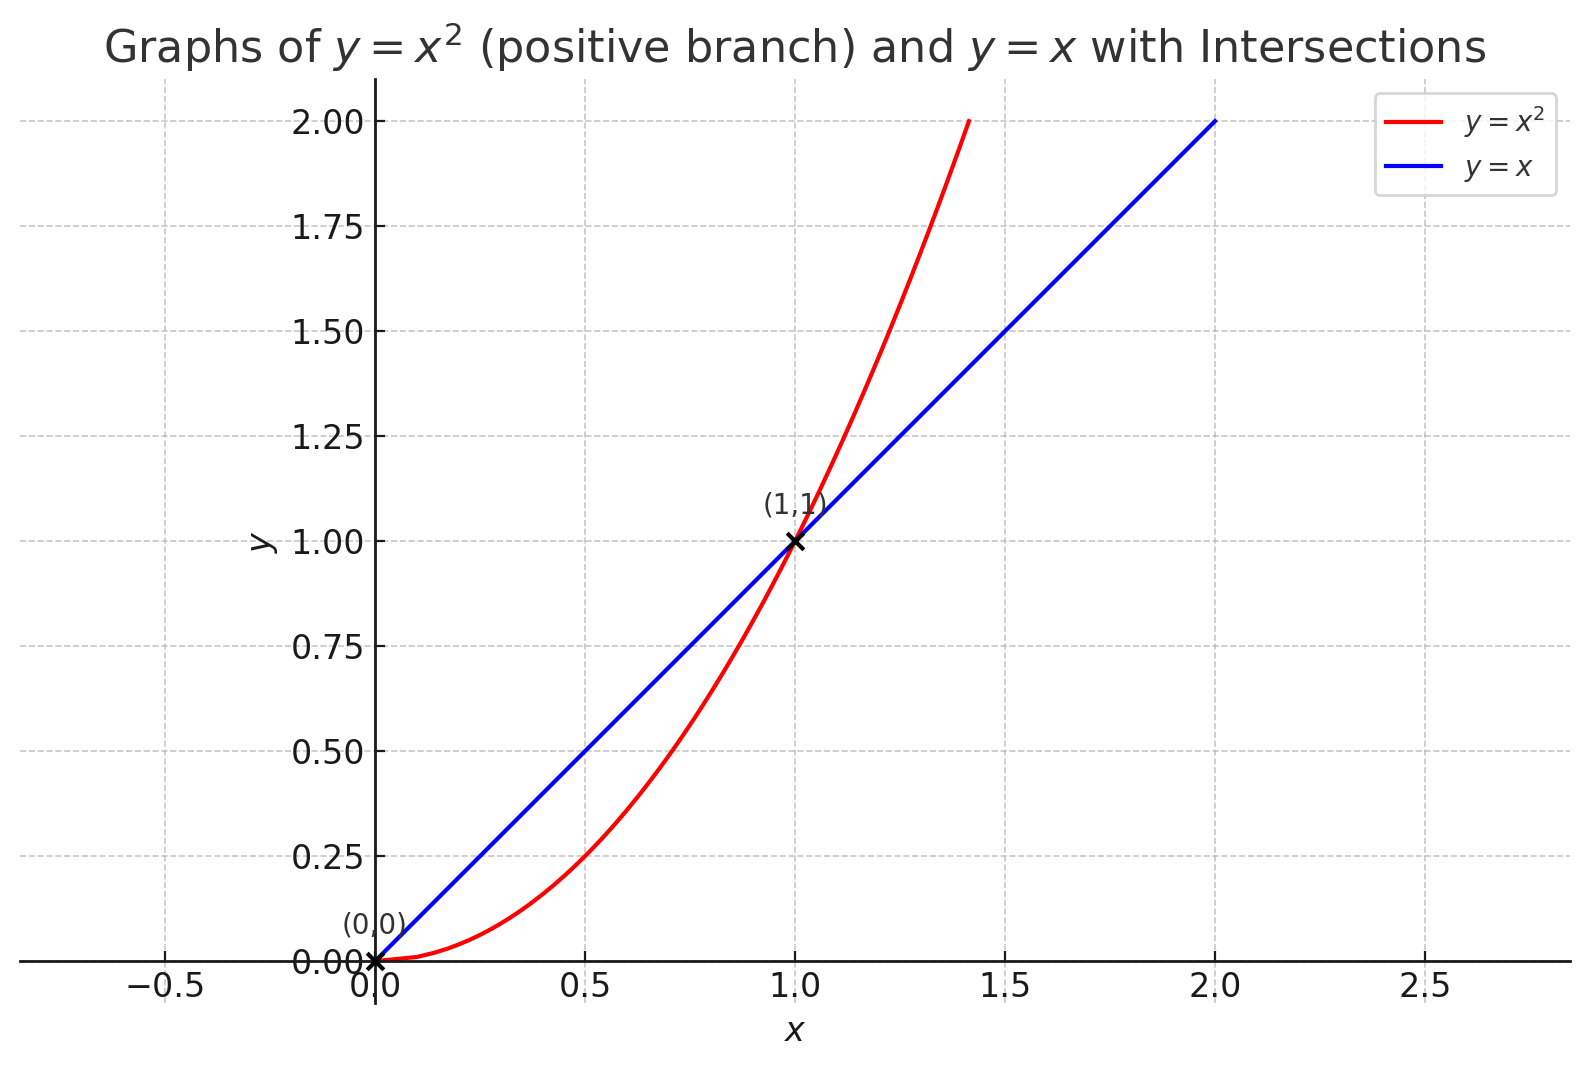
\includegraphics[width=\columnwidth, height=0.8\textheight, keepaspectratio]{figs/parabola_line.png}     
\end{frame}
\end{document}